\paragraph{Sơ đồ tuần tự luồng Xử lý tài liệu trong nền}
Luồng nghiệp vụ này mô tả
phần xử lý bất đồng bộ sau khi Document Service đã gửi Celery task \texttt{process\_document\_task(doc\_id)} vào RabbitMQ. Worker tiêu thụ task, tải file gốc từ R2, trích xuất nội dung, tạo summary, ghi vector chunks vào Milvus và cập nhật trạng thái tài liệu. Trong repo API hiện tại, phần đã thể hiện rõ là hợp đồng gửi task, các cờ trạng thái \texttt{has\_content}, \texttt{has\_summary} và các đường dẫn R2 tương ứng.

\begin{figure}[H]
\centering
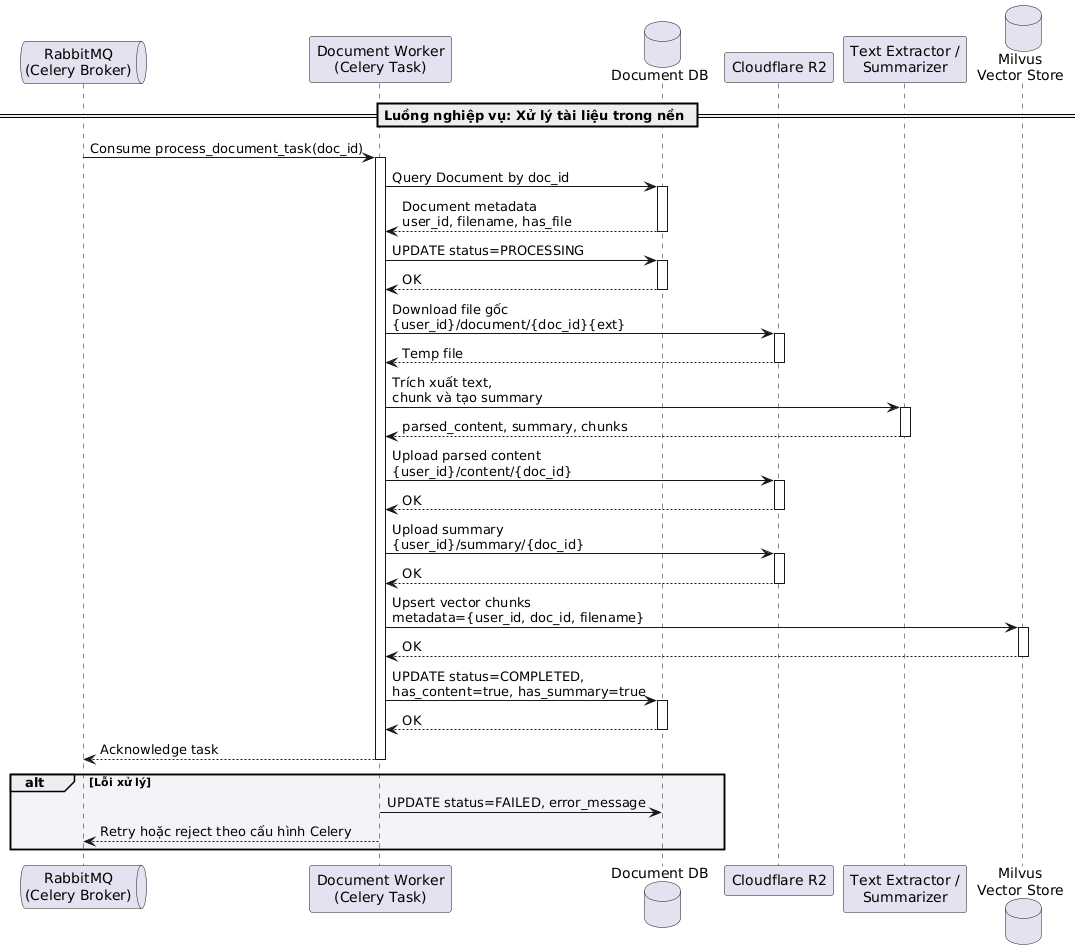
\includegraphics[scale = 0.18]{contents/Sequence/UML-Sequence-DocumentWorkerProcessDocument.png}
\caption{Sơ đồ tuần tự luồng Xử lý tài liệu trong nền}
\end{figure}

\subparagraph{Các thành phần tham gia}

\begin{table}[H]
\centering
\renewcommand{\arraystretch}{1.3}
\begin{tabular}{|l|l|p{5cm}|}
\hline
\textbf{Thành phần} & \textbf{Phân loại} & \textbf{Vai trò trong hệ thống} \\ \hline
RabbitMQ & Message Broker & Phân phối Celery task xử lý tài liệu cho worker. \\ \hline
Document Worker & Background Worker & Xử lý file, cập nhật trạng thái và ghi dữ liệu phục vụ RAG. \\ \hline
Document Database & Database & Lưu thông tin xử lý tài liệu. \\ \hline
Cloudflare R2 & Object Storage & Lưu file gốc, parsed content và summary. \\ \hline
Text Extractor / Summarizer & Processing Component & Trích xuất text, chia chunk và tạo summary. \\ \hline
Milvus & Vector Store & Lưu vector chunks theo user và document để truy vấn về sau. \\ \hline
\end{tabular}
\caption{Các thành phần tham gia luồng xử lý tài liệu trong nền}
\end{table}

\subparagraph{Mô tả tổng quan}
\begin{itemize}
\item Worker consume \texttt{process\_document\_task(doc\_id)} từ RabbitMQ/Celery.
\item Worker chuyển trạng thái tài liệu sang \texttt{PROCESSING}, tải file gốc từ R2.
\item Nội dung đã parse và summary được upload lại lên R2 theo \texttt{\{user\_id\}/content/\{doc\_id\}} và \texttt{\{user\_id\}/summary/\{doc\_id\}}.
\item Các chunk được embedding và upsert vào Milvus kèm metadata \texttt{user\_id}, \texttt{doc\_id}, \texttt{filename}.
\item Khi hoàn tất, Document được cập nhật \texttt{COMPLETED}, \texttt{has\_content=true}, \texttt{has\_summary=true}; nếu lỗi thì cập nhật \texttt{FAILED}.
\end{itemize}
